% Copyright (C) 2014-2017 by Thomas Auzinger <thomas@auzinger.name>

\documentclass[draft,final]{vutinfth} % Remove option 'final' to obtain debug information.

% Load packages to allow in- and output of non-ASCII characters.
\usepackage{lmodern}        % Use an extension of the original Computer Modern font to minimize the use of bitmapped letters.
\usepackage[T1]{fontenc}    % Determines font encoding of the output. Font packages have to be included before this line.
\usepackage[utf8]{inputenc} % Determines encoding of the input. All input files have to use UTF8 encoding.

% Extended LaTeX functionality is enables by including packages with \usepackage{...}.
\usepackage{amsmath}    % Extended typesetting of mathematical expression.
\usepackage{amssymb}    % Provides a multitude of mathematical symbols.
\usepackage{mathtools}  % Further extensions of mathematical typesetting.
\usepackage{microtype}  % Small-scale typographic enhancements.
\usepackage[inline]{enumitem} % User control over the layout of lists (itemize, enumerate, description).
\usepackage{multirow}   % Allows table elements to span several rows.
\usepackage{booktabs}   % Improves the typesettings of tables.
\usepackage[margin=0.5cm]{subcaption} % Allows the use of subfigures and enables their referencing.
\usepackage[ruled,linesnumbered,algochapter]{algorithm2e} % Enables the writing of pseudo code.
\usepackage[usenames,dvipsnames,table]{xcolor} % Allows the definition and use of colors. This package has to be included before tikz.
\usepackage{nag}       % Issues warnings when best practices in writing LaTeX documents are violated.
\usepackage{todonotes} % Provides tooltip-like todo notes.
\usepackage{hyperref}  % Enables cross linking in the electronic document version. This package has to be included second to last.
\usepackage[acronym,toc]{glossaries} % Enables the generation of glossaries and lists fo acronyms. This package has to be included last.
\usepackage{bm}

% Define convenience functions to use the author name and the thesis title in the PDF document properties.
\newcommand{\authorname}{Maximilian Sbardellati} % The author name without titles.
\newcommand{\thesistitle}{Interactive Exploded Views for Presenting DNA Nano-Structures} % The title of the thesis. The English version should be used, if it exists.

% Set PDF document properties
\hypersetup{
    pdfpagelayout   = TwoPageRight,           % How the document is shown in PDF viewers (optional).
    linkbordercolor = {Melon},                % The color of the borders of boxes around crosslinks (optional).
    pdfauthor       = {\authorname},          % The author's name in the document properties (optional).
    pdftitle        = {\thesistitle},         % The document's title in the document properties (optional).
    pdfsubject      = {Subject},              % The document's subject in the document properties (optional).
    pdfkeywords     = {a, list, of, keywords} % The document's keywords in the document properties (optional).
}

\setpnumwidth{2.5em}        % Avoid overfull hboxes in the table of contents (see memoir manual).
\setsecnumdepth{subsection} % Enumerate subsections.

\nonzeroparskip             % Create space between paragraphs (optional).
\setlength{\parindent}{0pt} % Remove paragraph identation (optional).

\makeindex      % Use an optional index.
\makeglossaries % Use an optional glossary.
%\glstocfalse   % Remove the glossaries from the table of contents.

% Set persons with 4 arguments:
%  {title before name}{name}{title after name}{gender}
%  where both titles are optional (i.e. can be given as empty brackets {}).
\setauthor{}{\authorname}{}{male}
\setadvisor{Assoc. Prof. Dr. Dipl.-Ing.}{Ivan Viola}{}{male}

% For bachelor and master theses:
\setfirstassistant{Dipl.-Ing.}{Haichao Miao}{}{male}

% For dissertations:
\setfirstreviewer{Pretitle}{Forename Surname}{Posttitle}{male}
\setsecondreviewer{Pretitle}{Forename Surname}{Posttitle}{male}

% For dissertations at the PhD School and optionally for dissertations:
\setsecondadvisor{Pretitle}{Forename Surname}{Posttitle}{male} % Comment to remove.

% Required data.
\setaddress{Rebengasse 35, 2700 Wiener Neustadt}
\setregnumber{01526262}
\setdate{02}{11}{2018} % Set date with 3 arguments: {day}{month}{year}.
\settitle{\thesistitle}{Interaktive Explosionsansichten zur Präsentation von DNA Nano-Strukturen} % Sets English and 

% Select the thesis type: bachelor / master / doctor / phd-school.
% Bachelor:
\setthesis{bachelor}
%
% Master:
%\setthesis{master}
%\setmasterdegree{dipl.} % dipl. / rer.nat. / rer.soc.oec. / master
%
% Doctor:
%\setthesis{doctor}
%\setdoctordegree{rer.soc.oec.}% rer.nat. / techn. / rer.soc.oec.
%
% Doctor at the PhD School
%\setthesis{phd-school} % Deactivate non-English title pages (see below)

% For bachelor and master:
\setcurriculum{Media Informatics and Visual Computing}{Medieninformatik und Visual Computing} % Sets the English and German name of the curriculum.

% For dissertations at the PhD School:
\setfirstreviewerdata{Affiliation, Country}
\setsecondreviewerdata{Affiliation, Country}


\begin{document}

\frontmatter % Switches to roman numbering.
% The structure of the thesis has to conform to
%  http://www.informatik.tuwien.ac.at/dekanat

\addtitlepage{naustrian} % German title page (not for dissertations at the PhD School).
\addtitlepage{english} % English title page.
\addstatementpage

\begin{acknowledgements*}
I want to thank Haichao Miao for being a great advisor, his continuous support and his valuable inputs. Additionally, I want to thank the staff of the Research Division of Computer Graphics, with special thanks to Hsiang-Yun Wu, for their feedback that showed me new ideas on how to improve my work. Last but not least, I want to thank my family, friends and colleagues for their support and advice. 
\end{acknowledgements*}

\begin{kurzfassung}
Mit der täglich steigenden Komplexität von DNA Nano-Strukturen, die mit der Unterstützung von Computern konstruiert werden, wird auch die Präsentation dieser komplexer.
Um das größte Problem bei der Präsentation, die visuelle Verdeckung von Stukturkomponenten, zu lösen, haben wir eine semi-automatische Methode entwickelt, die effektive interaktive Explosionsansichten von DNA Nano-Strukturen erstellt und besonders für Ausbildungszwecke eingesetzt werden kann.
Um dies zu bewerkstelligen, werden ausgewählte Komponenten einer DNA Nano-Struktur anhand der vier Parameter Explosionsrichtung, -distanz, -reihenfolge und Komponentenauswahl verschoben. In dieser Arbeit werden drei verschiedene Ansätze beschrieben, wie die Explosionsrichtung ausgewählt werden kann, wobei zwei davon von der Objektstruktur bestimmt sind und eine vom Benutzer willkürlich gewählt werden kann. Bei den zwei Struktur definierten Ansätzen wird eine Methode beschrieben wie man die Explosionsdistanz berechnen kann und drei verschiedene Explosionsreihenfolgen werden vorgestellt. Die Explosionskomponenten bei diesen zwei Ansätzen sind durch die hierarchische Struktur des Datensatzes bestimmt, das das Objekt beschreibt. Bei dem Ansatz, bei dem der Benutzer die Explosionsrichtung bestimmt, kann dieser auch die Explosionsdistanz und die Explosionskomponenten frei bestimmen. Dieser Ansatz stellt eine mögliche Explosionsreihenfolge zur Verfügung. Die entwickelte Applikation stellt außerdem die Möglichkeit bereit die Explosionen zu animieren und „Ease“ Funktionen in diesen Animationen zu verwenden.
\end{kurzfassung}

\begin{abstract}
As the complexity of computer-aided-designed DNA nano-structures progresses day by day, the presentation of these structures is becoming complex. To tackle the main presentation problem, visual occlusion of structure components, we developed a semi-automated method to create effective interactive exploded views for DNA nano-structures, especially for educational purposes. 
This is done by displacing selected components of a DNA nano-structure based on the four key parameters explosion direction, distance, order and component selection. 
In this thesis we describe three different strategies of choosing the explosion direction, with two of them being defined by the object structure and one by the user. For the two structure defined approaches a method to calculate the explosion distance and three different explosion orders is described. The explosion components for these two approaches are defined by the hierarchical structure of the dataset, that describes the object. The user defined approach lets the user decide on the explosion distance and features one possible explosion order. It also lets the user select the explosion components arbitrarily. The developed application additionally features the possibility to animate an explosion and to use easing in these animations.
\end{abstract}

% Select the language of the thesis, e.g., english or naustrian.
\selectlanguage{english}

% Add a table of contents (toc).
\tableofcontents % Starred version, i.e., \tableofcontents*, removes the self-entry.

% Switch to arabic numbering and start the enumeration of chapters in the table of content.
\mainmatter

\chapter{Introduction}
\label{chap:intro}

DNA nano-structures are the product of DNA nanotechnology, which uses DNA not for the purpose of carrying genetic information, but for the construction of arbitrary structures in a nanoscopic scale \cite{zhang2014structural}. 
As with all 3D structures, the presentation of DNA nano-structures on a 2D screen poses some challenges.
The two main challenges here are to control visual occlusion while also enhancing the visibility of the relationship between the different components of a structure.
DNA nano-structures often consist of several hundred components, which additionally are completely intertwined given the double helix form of DNA \cite{watson1953molecular}.
This makes the presentation of finished or work in progress DNA nano-structures in a visually appealing and understandable way even harder.

\par Out of the many different approaches to deal with visual occlusion (for an overview about occlusion management techniques see \cite{elmqvist2008taxonomy}), we chose the exploded view technique to overcome it in this particular case. 
An exploded view separates an object into different components before displacing them to reveal components that were occluded before.
Additionally it is used to enhance the visibility of the relationship between those components \cite{bruckner2006exploded}. 
This technique is especially suited to deal with visual occlusion when presenting DNA nano-structures, since it handles visual occlusion while still showing all the components of the exploded object. It also does not deform the individual components of an object and has features that enhance the visibility of component relationships.
Visual occlusion management techniques like transparency \cite{elmqvist2007employing} or X-ray tunnels \cite{bane2004interactive}, could also be fitting to handle visual occlusion for our problem statement. 
On the other hand techniques like adaptive cutaways \cite{burns2008adaptive}, deformations \cite{mcguffin2003using} or multiple viewports \cite{bares1998intelligent} are not suited for presenting DNA nano-structures in the way we want, since they do not show all the components, deform them and give no extra information about component relationships.

\par The aim of this thesis is to develop a method to use the exploded view technique for the presentation of DNA nano-structures. 
The focus in the development lies on creating an interactive framework that enables the user to create exploded views in a fast and easy way.
Above all, we aim to generate exploded views that are easily understandable and therefore can be used for educational purposes. 
The four parameters of an exploded view, that we consider in this thesis, are the explosion \textbf{direction}, explosion \textbf{distance}, explosion \textbf{order} and the \textbf{selection of the components}.

\section{DNA Nanotechnology}
\label{sec:mot}
DNA nanotechnology is a field that has been around for over 35 years. In the early 1980s Seemann et al. were the first ones to describe the use of the structural properties of DNA to construct nanoscale structures \cite{seeman1983design}. Since then the field has grown steadily, until in 2006 Rothemund developed the DNA origami technique \cite{rothemund2006folding}, which revolutionized the landscape of DNA nanotechnology and spread the interest in the field \cite{zhang2014structural}. Additionally, the arrival of simple computer aided design tools and simulation methods helped to boost the popularity of the field \cite{simmel2014wireframe}. In \autoref{fig:cubeAndTubeRotated_1} two exemplary DNA nano-structures are shown.

\begin{figure}
\centering
\begin{subfigure}{0.5\textwidth}
  \centering
  \includegraphics[width=\linewidth]{cube_1.png}
  \caption{DNA wireframe structure}
  \label{fig:cubeRotated_1}
\end{subfigure}%
\begin{subfigure}{0.5\textwidth}
  \centering
  \includegraphics[width=\linewidth]{hextube_2.png}
  \caption{DNA origami structure}
  \label{fig:tubeRotated_1}
\end{subfigure}
\caption{Two exemplary DNA nano-structures. The scaffold is marked grey and the staples are marked red.}
\label{fig:cubeAndTubeRotated_1}
\end{figure}

\par Some of the features that make DNA the exceptional building material or nanoscale structures that it is are its specific 3D conformation, chemical addressability, and its predictable Watson-Crick base-paring. The underlying concepts that allow the creation via self-assembly of objects or devices on a nanoscoping level with DNA, are branched DNA junctions and sequence-specific sticky end associations \cite{zhang2014structural}, \cite{seeman2007overview}. DNA nanotechnology can be applied to several use cases. The initial idea to build nanoscopic crystalline cages to orient other biological macromolecules soon lead to the notion of nanometer-scale robotics. Furthermore, concepts of DNA nanotechnology can be used for DNA-based computation and for the algorithmic assembly of materials \cite{seeman2007overview}, \cite{winfree1996computational}.

\par Most of the DNA nano-structures that we used to develop and test our approach were designed and built using the DNA origami technique. Such structures consist of one long \textbf{scaffold strand} and a number of \textbf{staple strands} that provide the Watson-Crick complements for the scaffold. A shown in \autoref{fig:dnaOrigami}, by designing the staples in the correct way, the scaffold can be folded to form the desired shape by creating periodic crossovers, that hold the whole structure together \cite{rothemund2006folding}.

\begin{figure}
\centering
\includegraphics[width=0.5\linewidth]{roth_dna_origami.png}
\caption{A finished DNA origami design. The scaffold (black) is folded by the staples (red, green, blue, yellow) \cite{rothemund2006folding}.}
\label{fig:dnaOrigami}
\end{figure}

\section{Exploded Views}
\label{sec: explV}

Exploded views have been used to deal with the problem of visual occlusion for centuries. One of the earliest examples is an exploded view drawing by Leonardo da Vinci that is shown in \autoref{fig:davinci}. The most common use cases for exploded views in the last 5 centuries were construction manuals, architectural plans and drawings in the field of biology and medicine, all with the goal of showing all the parts of the illustrated object concurrently and making the relationship between these parts understandable. Today the use cases are still the same, but in a far more advanced way. The rise of personal computers with graphical user interfaces, in combination with new methods of data acquisition, like medical data acquired from computer tomography or the design of mechanical parts with computer-aided design, created an environment that revolutionised the design of exploded views.
\par With these new technologies, exploded views did not need to be drawn by hand anymore, but rather could be designed in an interactive way on a computer, or even generated completely automatically. The first attempts to do so were made in the late 1980s and early 1990s by various research groups \cite{de1987simplified}, \cite{kroll1989rule}, \cite{mohammad1993automatic}, with most of them using graph based approaches. The current state of the art and some different approaches on how to create exploded views are discussed in further detail in Chapter \ref{chap:relWork}.

\begin{figure}
\centering
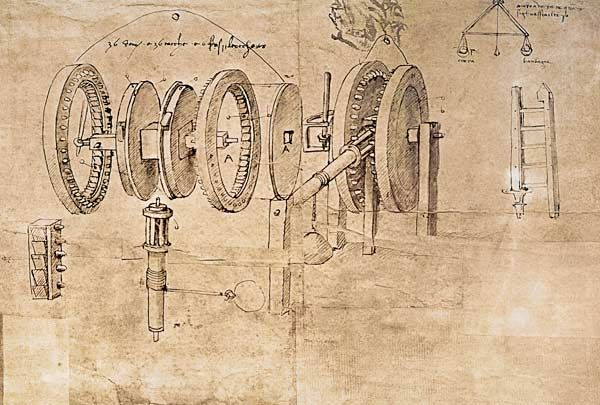
\includegraphics[width=0.7\linewidth]{DaVinciExplodedView.jpg}
\caption{Exploded view of a gear assembly, from Leonardo da Vinci’s Codex Atlanticus (15th century).}
\label{fig:davinci}
\end{figure}

\section{Methodological Approach}
\label{sec:methodApp}
The goal of this thesis is to generate exploded views for DNA nano-structures to facilitate their presentation. For this purpose we developed different explosion styles to be able to generate expressive exploded views for a wide range of DNA nano-structures.

\par In this thesis we present the \textbf{structure-defined explosion} and the \textbf{user-defined-path explosion}. In the structure-defined explosion, the explosion distance is calculated using the current DNA nano-structure. For calculating the explosion direction, we introduced two different sub-styles of the structure defined explosion, the spherical explosion and the principal component explosion. The spherical explosion uses the vector from the parent structure center to the center of of the explosion component as the explosion direction, which has the convenient effect that such an explosion preserves the initial from of the structure (see \autoref{fig:cubeAndCubeExploded_1}). The principal component explosion uses PCA (Principal Component Analysis \cite{jolliffe2011principal}) to calculate the three principal components of a DNA nano-structure, using the 3D position of all its atoms, which then serve as the explosion directions for the explosion components.
\par The user-defined-path explosion lets the user decide on the explosion distance and direction. The user can draw arbitrary paths along which the explosion components explode.

\begin{figure}
\centering
\begin{subfigure}{0.5\textwidth}
  \centering
  \includegraphics[width=\linewidth]{cube_2.png}
  \caption{DNA wireframe cube}
  \label{fig:cube_1}
\end{subfigure}%
\begin{subfigure}{0.5\textwidth}
  \centering
  \includegraphics[width=\linewidth]{cube_exploded_1.png}
  \caption{Exploded view of the DNA wireframe cube}
  \label{fig:cubeExploded_1}
\end{subfigure}
\caption{The exploded view of the DNA wireframe cube (\autoref{fig:cubeExploded_1}) is generated by using the spherical explosion on the staples and the scaffold. The structural form of the cube is still recognizable in the exploded view.}
\label{fig:cubeAndCubeExploded_1}
\end{figure}


\section{Structure of the Work}
\label{sec:struct}
This bachelor thesis is structured as follows: In Chapter \ref{chap:relWork} an overview of the state of the art in the field of generating exploded views is given with special focus on approaches that are related to ours. Different use cases for generating exploded views are introduced and the features of exploded views that make it suitable for this work are explained. Chapter \ref{chap:method} dives into the different explosion styles, that are introduced in this work. The structure defined explosions, spherical explosion and principal component explosion, and the user-defined-path explosion are explained in detail. Chapter \ref{chap:impl} gives a closer look into the implementation of these styles and introduces some overarching features that effect all of the explosion styles. Chapter \ref{chap:result} shows and discusses the results of this work. Some possible enhancements are discussed in Chapter \ref{chap:openI}. The thesis is concluded in Chapter \ref{chap:summary}.

\chapter{Related Work}
\label{chap:relWork}

In recent years numerous works have been published in the field of exploded views. In this chapter the approaches that have an impact on our work in this thesis are introduced.

\par Agrawala et al. \cite{agrawala2003designing} used exploded views to design effective assembly instructions in 2003. To achieve this they developed a series of design principles to follow when designing assembly instructions. One of these design principles states that structural diagrams are inferior to action diagrams. Structural diagrams show all assembly parts that should be attached to the object in each assembly step already in their ultimate position. Action diagrams on the other hand show the parts that need to be attached in each step, while being spatially separated from the rest of the object and featuring lines that illustrate the correct way of attachment. Another principle deals with the use of hierarchy and the grouping of parts. It states that people think about assemblies considering the hierarchy of the parts. Parts with similar characteristics are often seen as a group and parts within such a group should be added to the assembly in a parallel or sequential way. This is comparable to the way we use hierarchy and explosion orders in this thesis.

\par Li et al. \cite{li2008automated} developed a system to generate interactive 3D exploded view diagrams of complex mechanical 3D models. They followed a set of conventions for illustrating mechanical assemblies and applied them to their interactive explosion diagrams. One of these conventions introduces a blocking constraint, which means that a part can only explode if there is no other part blocking its way. To work effectively with this constraint Li et al. introduce an explosion tree which sorts the parts according to the blocking constraint. Parts that are not blocked by any other parts are found in the leafs of the tree and explode first. In some cases this method is not sufficient, the most common being when one part contains other parts. In this case, the container is split into two segments and those segments are exploded. To split it, a cutting plane is used, which passes through the bounding box center of the container. The normal of the cutting plane is parallel to the chosen explosion direction. To satisfy the convention of compactness the plane is chosen to minimize the distance the segments must be separated to show the internal parts. Even though the blocking constraint add a lot of realism to an interactive exploded view, we discard it in our approach for the sake of simplicity.
\\Li et al. \cite{li2008automated} also focus heavily on the interactive exploration of 3D models. The expansion and collapse of an exploded view can be \textbf{animated}. It is also possible to directly manipulate parts by dragging them. To enforce the blocking constraint while dragging a part, the offset to the explosion ancestors of the part in the explosion tree is propagated. Another interaction feature enables the user to automatically expose targeted parts. The user selects one part as target and the system generates an exploded view, that explodes all parts that occluded the target (see \autoref{fig:turbine}).

\par Sonnet et al. \cite{sonnet2004integrating} presented an approach to integrate annotations to explosion diagrams, for the purpose of exploring virtual 3D models. The two main parts of their work are the interactive creation of explosion diagrams and the visually appealing presentation of accompanying text for exploded model components. For exploring 3D models they use a 3D probe that displaces model components when they are covered by the probes scope, similar to Elmqvist's BallonProbe \cite{elmqvist2005balloonprobe} (see \autoref{fig:balloon}). To decide if a component is inside the probes scope or not, a representative point of the component need to be determined. They propose three different approaches to calculate this representative point. The simplest one is to use the center of the components bounding box, which has the drawback that this point might be located outside the component. A more sophisticated way is to calculate the skeleton of the component and determine a significant point on the skeleton as representative. Usually the point at which the most branches of the skeleton coincide is chosen. Since this point may be far away from the component center, this approach is also not perfect. A compromise between the two mentioned approaches is to use the point of the skeleton which is nearest to the bounding boxes center. This point is also referred to as centroid of the component. The approach we use to calculate a representative point for the explosion components is introduced in Chapter \ref{chap:impl}.

\par The BalloonProbe of Elmqvist \cite{elmqvist2005balloonprobe} greatly inspired the way we use spherical explosion in our work. Elmqvist states that the problem of visual occlusion can be separated into two parts, \textbf{object discovery} and \textbf{object access}. He defines object discovery as the problem of finding all objects that are currently displayed and object access as retrieving all the graphically encoded information of an object. Since one cannot retrieve any object information, if one does not even know the object exists, object discovery is the severer problem. Object access is also affected by partial object occlusion. According to Elmqvist, both of these problems can be solved with his BalloonProbe approach. As can be seen in \autoref{fig:balloon}, he defines a balloon around the cursor. Every object that falls into the balloon gets projected onto the balloon surface along the vector passing from the balloon center through the center of the displaced object, which is similar to the approach of Sonnet et al. \cite{sonnet2004integrating}. On the surface, the object gets drawn normally to its old position. To keep a sense of the original object positions, a wireframe version of the objects is rendered at their original position. It is also possible to select a group of objects that should not be displaced, even if they are inside the balloon. This feature is very effective in dealing with the object access problem, since it displaces all but some selected objects to then make it possible to retrieve all their graphically encoded information.

\begin{figure}
\centering
\begin{subfigure}{0.45\textwidth}
  \centering
  \includegraphics[width=\linewidth]{balloonProbe.png}
  \caption{2D overview of the BalloonProbe technique. Components that are inside the BallonProbes scope get projected spherically onto the probes surface \cite{elmqvist2005balloonprobe}.}
  \label{fig:balloon}
\end{subfigure}%
\begin{subfigure}{0.5\textwidth}
  \centering
  \includegraphics[width=\linewidth]{turbine.png}
  \caption{This illustration of a turbine model was automatically computed to expose the user-selected target part labeled in red \cite{li2008automated}.}
  \label{fig:turbine}
\end{subfigure}
\caption{The BalloonProbe technique (\autoref{fig:balloon}) inspired the spherical explosion. \autoref{fig:turbine} shows an exploded view, where the outer shell and the exhaust housing are split into two parts, similar to the PCA explosion.}
\label{fig:ballonAndTurbine}
\end{figure}


\chapter{Explosion Styles}
\label{chap:method}
As stated before, there are two different explosion styles for DNA nano-structures that we present in this thesis: the structure-defined explosion and the user-defined-path explosion. The structure-defined explosion features two sub-styles: the spherical explosion and the principal component explosion. In this chapter the methodology of these styles is introduced in detail by examining how the parameters explosion order, explosion direction, explosion distance and the selection of the explosion components in regard to an exploded view are handled by each of the explosion styles.

\section{Structure-Defined Explosion}
\label{sec:methodGuided}
The structure-defined explosion derives all its parameters from the data hierarchy and the 3D relationship and position of the components of the explosion object itself. The two sub-styles, the spherical explosion and the principal component explosion, compute three of the four major explosion parameters in the same way. 
Only the approach of determining the explosion direction differs from style to style.

\subsubsection{Selection of Components}
\label{subsubsec:explcompsStruc} 
As seen in \autoref{fig:samsonStruct}, the data we work with is already structured in a hierarchical way. 
The structure-defined explosion uses a parent-child relationship to handle the selection of explosion components. The user first has to select a parent level that is also present in the actual data. 
The afterwards selected child level has to be lower in the hierarchy, than the parent level. If, for example, \(molecule\) is chosen as the parent level, one could choose \(residue\) as the child level. 
In this approach, we consider each parent as an individual explosion object and the children as the explosion components of the corresponding parent. 
Therefore, to calculate the parameters explosion order, explosion distance and explosion direction for an explosion child, only the structure of its parent is taken into account. 
Since the procedure of creating an exploded view is the same for each parent structure, it is described assuming that we only have one parent.

\par In the following elaborations we refer to the explosion components as children. Since parents and children most of the time are not atoms, the lowest hierarchical level, we need to establish a representative point when we use the position of a parent or child for calculations. In our approach, we use the center of the parent or child structure which is calculated by determining the average 3D position of all the atoms in the structure as the representative point.

\begin{figure}
\centering
\includegraphics[width=0.5\linewidth]{SAMSON_structure.png}
\caption{Example structure of a molecule. M = molecule, C = chain, R = residue, B = backbone, SC = sidechain}
\label{fig:samsonStruct}
\end{figure}

\subsubsection{Explosion Order}
\label{subsubsec:explOrderStruc}
Structure-defined explosion allows the user to choose between three different explosion orders: parallel, peeling and sequential (see \autoref{fig:explOrders}). 
It is also always possible to select one or more explosion children, in which case only these children explode. All the steps needed to prepare for the selected explosion order are done in preprocessing after the explosion level was chosen. Since the parallel explosion is a special form of the peeling explosion, we first take a closer look at peeling, before explaining parallel explosion.

\begin{figure}
\centering
\begin{subfigure}{0.3\textwidth}
  \centering
  \includegraphics[width=\linewidth]{cube_chain.png}
  \caption{Original Structure}
  \label{fig:chainParExpl}
\end{subfigure}%
\begin{subfigure}{0.3\textwidth}
  \centering
  \includegraphics[width=\linewidth]{cube_chain_exploded.png}
  \caption{Parallel Explosion}
  \label{fig:chainParExpl}
\end{subfigure}%

\medskip

\begin{subfigure}{0.3\textwidth}
  \centering
  \includegraphics[width=\linewidth]{cube_chain_exploded_peel_halfway.png}
  \caption{Peeling Explosion}
  \label{fig:chainPeelExpl}
\end{subfigure}%
\begin{subfigure}{0.3\textwidth}
  \centering
  \includegraphics[width=\linewidth]{cube_chain_exploded_seq_halfway.png}
  \caption{Sequential Explosion}
  \label{fig:chainSeqExpl}
\end{subfigure}
\caption{The three explosion orders using spherical explosion on a chain of the DNA wireframe cube. In \autoref{fig:chainParExpl} all residues of this chain are exploding simultaneously. In \autoref{fig:chainPeelExpl} the peeling group that is currently exploding is marked yellow. \autoref{fig:chainSeqExpl} shows the sequential explosion. The residues that are currently exploding are marked yellow.}
\label{fig:explOrders}
\end{figure}

\par The idea behind \textbf{peeling} is to group the children of each parent according to the distance they have to their parents center and then explode one group after another starting with the group farthest away. The children within a group explode simultaneously. The number of groups can be chosen by the user. This approach is useful if one wants to take a closer look at parts of the structure that are occluded, without exploding every component and instead, only removing parts that hinder the visibility of specific parts.. The first parameter we need to determine is the length of the peeling interval (see \autoref{fig:peeling}). This is done by subtracting the distance of the nearest child to the parent, \(min\), from the distance of the farthest away child to the parent, \(max\), and dividing it by the number of peeling groups, \(n\), as shown in \autoref{eq:peelInterval}.

\begin{equation}
\label{eq:peelInterval}
peelingIntervalLength = \frac{max - min}{n}
\end{equation}

The next step is to assign the children to the correct group by iterating through the group indices $g$ and children and checking if $ (g - 1) \cdot peelingIntervalLength < x_i - min <= g \cdot peelingIntervalLength$, with $x_i$ being the distance of the current child $i$ to the parent. At last, the peeling groups are sorted in descending order according to their distance to the parent center.

\begin{figure}
\centering
\includegraphics[width=0.9\linewidth]{peeling.png}
\caption{2D overview of the grouping into the correct peeling groups. The black dot represents the center of the parent structure. The gray dots represent the center of the parents children. The distance between the nearest and the farthest away child gets divided into three intervals of the same length. The children get grouped according to the interval they lay in. The groups explode starting with the farthest away group, group 3 in this case, and all the children in the same group explode simultaneously.}
\label{fig:peeling}
\end{figure}

\par When using \textbf{parallel explosion}, all children explode simultaneously. 
This is a fast way to create a completely exploded representation of the object which can be used to get a quick overview of the objects components. 
On the other hand, it is hard to see how different parts of the objects interact with each other, because they all move at the same time. 
Since it has the same behaviour as a peeling explosion with just one peeling group, the number of peeling groups is set to 1 and the explosion is carried out like a peeling explosion, when the user chooses the parallel explosion in the GUI.

\par The third possible explosion order is \textbf{sequential}. 
The idea behind the sequential explosion is to explode one child after another starting with the child that is farthest away from the parent center. 
This is done by sorting the children in descending order by their distance to the parent center and then exploding one by one. 
This explosion order has the benefit of highlighting the interaction of the part that is currently moving with its surrounding parts. 
Especially when animated, this approach gives an excellent overview on how each part fits into the whole object.

\subsubsection{Explosion Distance}
\label{subsubsec:expldistStruc}
The last parameter that is attained equally by the spherical and the principal component explosion is the \textbf{explosion distance}. 
Since we do not want to shift the explosion components an arbitrary or fixed distance, we developed an approach that calculates the explosion distance $d_i$ for each child $i$ based on four explosion distance parameters:

\begin{equation}
\label{eq:d}
d_i = e \cdot f \cdot s \cdot p_i
\end{equation}

The \textbf{explosion value} \(e\) is a value normalized between 0 and 99. 
This parameter is adjusted by the user by manipulating a slider and represents the main source of changing the explosion distance interactively. 
The \textbf{force parameter} \(f\) is also adjustable by the user via a slider and shortens or lengthens the maximal explosion distance. 
The slider features the natural numbers from 0 to 10. 
If the chosen slider position is between 0 and 5 the value gets normalized and if it is between 5 and 10 it gets projected to the interval 1-3. 
This enables the user to extend the maximum explosion distance to up to three times the original maximum value of \(d_i\). 
The \textbf{structural parameter} \(s\) ensures that the explosion distance for smaller objects is less than for larger objects. 
It is calculated in a preprocessing step by determining the average distance of all atoms of an object in an unexploded state to its center which is then divided by a given constant \(sD\):
\begin{equation}
\label{eq:s}
s = \frac{averageDistanceToObjectCenter}{sD}
\end{equation}
We chose \(sD\) to be 25 in our implementation, because it delivered the most pleasing results.
The last of the four parameters that influence the explosion distance is the \textbf{position parameter} \(p_i\). 
It represents the relative distance of an explosion child to the center of the parent structure. 
This is also done in preprocessing by first determining the distance of the child that is farthest, and the one that is nearest from the parent to the parent in an unexploded state. 
In a second iteration the position parameter for the explosion child is calculated by normalizing the distance of the current explosion child $i$ to the parent \(x_i\) in the interval between the farthest, \(max\), and the nearest, \(min\), child to the parent, as shown in \autoref{eq:p}.

\begin{equation}
\label{eq:p}
p_i = \frac{x_i - min}{max - min}
\end{equation}

Unlike the other parameters that have the same effect on every explosion child of a parent structure, \(p_i\) has a different value for each child $i$ and has the effect that children that are nearer to the parent center, have a shorter explosion distance than children that are further from the center. As seen in \autoref{fig:posCoeffEffect}, this effect also preserves the underlying form of the object even in its exploded state. When working with objects that have a more linear or tube-like structure, this effect is sometimes not desirable since it hinders children nearer to the center to explode far enough. Therefore, it is also possible to omit the position parameter and calculate the explosion distance using only the other three parameters.

\begin{figure}
\centering
\begin{subfigure}{0.3\textwidth}
  \centering
  \includegraphics[width=\linewidth]{cube_chain.png}
  \caption{}
  \label{fig:chainNotExploded}
\end{subfigure}%
\begin{subfigure}{0.3\textwidth}
  \centering
  \includegraphics[width=\linewidth]{cube_chain_exploded.png}
  \caption{}
  \label{fig:chainPosCoeff}
\end{subfigure}%
\begin{subfigure}{0.3\textwidth}
  \centering
  \includegraphics[width=\linewidth]{cube_chain_noPosCoeff.png}
  \caption{}
  \label{fig:chainNoPosCoeff}
\end{subfigure}
\caption{\autoref{fig:chainNotExploded} shows a chain of the DNA wireframe cube. In \autoref{fig:chainPosCoeff} the chain is exploded on the residue level considering the position parameter. The underlying form of the chain is preserved. \autoref{fig:chainNoPosCoeff} does not consider the position parameter. Therefore, each residue has been moved exactly the same distance and the underlying form gets distorted. Both explosions use the spherical explosion.}
\label{fig:posCoeffEffect}
\end{figure}

\subsection{Spherical Explosion}
\label{subsec:methodSphere}
The idea behind the spherical explosion is similar to the balloon probe of Elmqvist \cite{elmqvist2005balloonprobe} in terms of how the \textbf{explosion direction} is determined by the vector from the center of the balloon probe to the component that gets moved. In our case, we did not use the center of the balloon probe, but the center of the parent structure and the component to establish the explosion direction. Additionally the explosion distance is calculated as described in Subsection \ref{subsubsec:expldistStruc} instead of projecting all the explosion components onto a sphere with a given radius.

\par To determine the explosion direction of a child $i$ the center of the parent $pc$ is saved in a preprocessing step. Additionally, the original distance $do_i$ from the parent center to the child is saved. When the user is manipulating the sliders to explode an object, the calculated explosion distance $d_i$ is added to $do_i$:
\begin{equation}
\label{eq:du}
du_i = do_i + d_i
\end{equation}
with $du_i$ being the updated distance from the parent center to the child. In the next step, the current center of the child $c_i$ is calculated to determine its current 3D position. Next, the vector from the parent center to the child center $\bm{\vec{v}} = c_i - pc$ is calculated and normalized. The updated position of the child $cu_i$ after being exploded is then determined by extending $\bm{\vec{v}}$ per $du_i$. Since $\bm{\vec{v}}$ starts at the origin and not at the parent center, $\bm{\vec{v}}$ is moved back to $pc$:
\begin{equation}
\label{eq:cuSphere}
cu_i = \bm{\vec{v}} \cdot du_i + pc
\end{equation}
To move the child to its new position, the vector from $c_i$ to $cu_i$ is calculated and added to the position of every atom of the child. 

\par The spherical explosion achieves its visually most appealing results when used on objects that have similar length in all 3 dimensions. If that is the case, as with the DNA wireframe cube or the DNA wireframe icosahedron (see \autoref{fig:res_ico}), the resulting exploded views are easy to understand and the preservation of the underlying object from can be seen in a perspicuous way.


\subsection{Principal Component Explosion}
\label{subsec:methodPCA}
The principal component explosion uses aspects of PCA (principal component analysis \cite{jolliffe2011principal}) to determine the \textbf{explosion direction}. Most of the time PCA is used to explore large datasets and for making predictive models. The so called principal components refer to the \textbf{eigenvectors} of the covariance matrix of the given dataset, which in our case consist of the given DNA nano-structures atom-positions. We use them to determine possible explosion directions. The maximum number of principal components in a dataset is defined as $min(n-1,p)$, with $n$ being the number of observations and $p$ the number of variables each observation has. In our case, the observations are the positions of the explosion components (children of a given parent structure), which have three variables (their x,y and z coordinates). Therefore, we can compute a maximum of three possible explosion directions. The first principal components has the highest possible variance given a dataset and is the longest of the eigenvectors. The following components have the largest variance that is still possible given the constraint of being orthogonal to the already established components.

\par The three possible explosion directions are calculated in a preprocessing step. First, the position of each child in an unexploded state $c_i$ is saved and the center of the parent, which is equivalent to the mean of all its children, is calculated. Next, the covariance matrix is computed and its eigenvectors are calculated. The eigenvectors are sorted in descending order according to their length before being normalized and saved.

\par When choosing the principal component explosion, the user has to choose along which eigenvector $e_x, x \in \{1,2,3\}$ he wants to explode. If the explosion sliders are the manipulated, the chosen eigenvector $e_x$ for each child $i$ is extended to the length of the calculated explosion distance $d_i$. Since we do not want to move all children in the same direction, a plane is laid through the parents center which is orthogonal to $e_x$. If a child lies on the backside of the plane, the extended eigenvector is subtracted from $c_i$ and if it lies on the front of the plane, it gets added to $c_i$ to calculate the updated position of the child $cu_i$: 
\begin{equation}
\label{eq:cuPCA}
cu_i = c_i \pm (e_x \cdot d_i)
\end{equation}
To move the child to its new position, the vector from the current child center to $cu_i$ is calculated and added to the position of every atom of the child. 
\\ The principal component explosion provides visually appealing and understandable exploded views with objects of all shapes.

\section{User-Defined-Path Explosion}
\label{sec:methodPath}
Instead of deriving all the explosion parameters from the structure of the explosion object itself, as in the structure-defined explosion, the user-defined-path explosion lets the user define most of them arbitrarily.
The idea behind this approach is to give the user more freedom in designing his individual exploded views.
When the user has selected the components he wants to explode, the explosion direction and distance are set by creating an arbitrary explosion path, using arrows that can be drawn directly in the view-port.
This gives the user the opportunity to create complex exploded views and animations (see \autoref{fig:pathExample}).

\begin{figure}
\centering
\includegraphics[width=0.7\linewidth]{hextube_path_2.png}
\caption{User-defined-path explosion of a DNA origami structure. Two chains of the structure were chosen as explosion groups. Each group has an explosion path consisting of 2 arrows (green and blue). The groups are not fully exploded.}
\label{fig:pathExample}
\end{figure}

\subsubsection{Selection of Components}
\label{subsubsec:explcompsPath} 
In user-defined-path explosion, the structure of the object is not considered when selecting the explosion components.
Instead, one can select an arbitrary group of atoms from the object and mark them as an explosion group.
The only constraints when adding a new group are that it is not allowed to be empty or contain atoms that are already members of another explosion group, since an atom cannot explode in more than one direction at a time.
If one still wants to use the given structure of the object, it is possible to select a node from the object hierarchy (see \autoref{fig:samsonStruct}) and add it as explosion group, as long as the constraints are not violated.
If a group consist of more than one atom a representative point is needed when talking about the groups position. Similar to the structure-defined explosion in Section \ref{sec:methodGuided}, we use the center of the explosion group as its representative.
It is also possible to delete existing explosion groups.

\subsubsection{Explosion Order}
\label{subsubsec:explOrderPath}
This approach only features the \textbf{parallel explosion} order. When the user manipulates the explosion slider every explosion group explodes simultaneously. It is also possible to select one or more groups manually. In this case, only the selected groups explode.

\subsubsection{Explosion Distance and Direction}
\label{subsubsec:expldistdirPath}
The \textbf{explosion distance} and \textbf{direction} are defined by the path that the user draws into the view-port. 
An explosion groups path consists of up to 5 arrows, the first one starting at the center of the group and ending wherever the user clicks in the view-port. 
The following arrows always start at the end of the previous one. 
Once a path is drawn, the group explodes along the \textbf{direction} that is set by the path.
The maximum \textbf{explosion distance} is defined by the paths length, therefore each group has a different maximum explosion distance. The actual explosion distance $d$ is interactively manipulated via a slider in the user interface.

\par When a group is created, an empty path is generated.
Additionally, a new path model $m$ is created that contains the start $s$ and end atom $e$ of each arrow that is drawn for this path as seen in \autoref{fig:SAMSONpaths}. 
This is done to enable the \textbf{manipulation} of the arrow after it is drawn by changing the position of the arrows atoms.
The first arrow of the path is the only one that creates a start and an end atom. 
The following arrows use a reference to the end atom of the previous arrow as their $s$ and only create a new $e$ for themselves.
Each arrow $i$ is represented by a tuple $al_i = (s_i,e_i,l_i)$ which is saved in a vector, the first arrows tuple being the first element of the vector. 
$l_i$ represents the length of the arrow.
When deleting arrows from a path, it is only possible to delete them from the last one to the first one, otherwise it would cut the path into two or more separated parts. 
Deleting an arrow also deletes the last atom from $m$ and if the first arrow gets deleted, its start atom also gets deleted.

\begin{figure}
\centering
\begin{subfigure}{0.4\textwidth}
  \centering
  \includegraphics[width=0.9\linewidth]{SAMSON_paths.png}
  \caption{Path nodes in the menu.}
  \label{fig:SAMSONpathStruc}
\end{subfigure}%
\begin{subfigure}{0.4\textwidth}
  \centering
  \includegraphics[width=0.9\linewidth]{hextube_path_gold.png}
  \caption{Path nodes in the view-port.}
  \label{fig:pathsGold}
\end{subfigure}
\caption{When a group gets created, a new path model for the path is generated. The first drawn arrow creates 2 atoms describing its start and end. The following arrows use the end atom of the previous arrow as start atom and create an end atom for themselves. By moving the atoms, the direction and distance of the path can be manipulated.}
\label{fig:SAMSONpaths}
\end{figure}

To actually move an explosion group to its exploded destination, the groups position on its path need to be determined. 
First, the percentage the slider is moved is calculated by dividing $d$ with its maximum value of the slider. 
Next, the total length of the path $t$ is determined by adding the length of all its arrows. 
By multiplying the percentage of the slider with $t$, we compute at which length of the path the group needs to be moved $t'$. 
To get the 3D position on the path, first we need to find the arrow on which the group lands.
To do so, we iterate over the arrows, starting with the first one, and subtract each arrows length from $t'$:
\begin{equation}
\label{eq:t_path}
t' = t' - l_i
\end{equation}

When $t'$ gets negative we have found the correct arrow $x$.
By reversing the last subtraction and diving $t'$ by $l_x$, we get the percentage $p$ of $l_x$ where the group hast to move:
\begin{equation}
\label{eq:p_path}
p = \frac{t' + l_x}{l_x}
\end{equation}

Next, the vector $\bm{\vec{v}}$ from $s_x$ to $e_x$ is calculated and resized to the needed length by multiplying it with $p$.
At the end, $\bm{\vec{v}}$ is translated back to the arrows beginning by adding the arrows start position to $\bm{\vec{v}}$, which now points to the exact location that the group needs to explode to.

\par To move the group to its new position, the position of the groups center is subtracted from $\bm{\vec{v}}$ and the result is added to the position of every atom of the group. An example of a complex user-defined-path explosion is shown in \autoref{fig:res_tube}.


\chapter{Implementation}
\label{chap:impl}
In this chapter, the implementation of the styles for exploding DNA nano-structures that were introduced in detail in Chapter \ref{chap:method} are described. First, we introduce the application in which the exploded views for DNA nano-structures can be used. Additionally, the programming language and the used frameworks are mentioned. Then the implementation of each explosion style on its own is discussed by examining how each style is integrated in the application starting from the GUI (graphic user interface). We also take a closer look at additional features that support each style or work overarching with multiple styles.

\section{Software and Hardware}
\label{sec:soft}
\par As the major development environment, Visual Studio 2015 was used on a Windows 10 platform.
C++14 was used as the main programming language.
The GUI was programmed with Qt 5.10.1 using Qt Creator 4.6 for the design and the msvc2015-64 Compiler. 
The application was developed as an element for SAMSON: Software for Adaptive Modeling and Simulation Of Nanosystems version 0.6\footnote{https://www.samson-connect.net}. The SAMSON SDK version 0.6 with the provided API\footnote{https://documentation.samson-connect.net/developers/latest/} was used to interact with the SAMSON software platform.
To calculate the eigenvectors for the principal-component explosion (see Subsection \ref{subsec:methodPCA}), the header only library eig3 by Barnes\footnote{http://barnesc.blogspot.com/2007/02/eigenvectors-of-3x3-symmetric-matrix.html} was used.

\par The hardware configuration used for testing and creating the results (see Chapter \ref{chap:result}) was comprised of the following main components: 
\\ Intel(R) Core(TM) i7-7500U CPU @2.70GHz 2.90GHz
\\ 16 GB RAM
\\ NVIDIA GeForce 940MX


\subsection{Application Structure}
\label{subsec:appStruct}
The core of the explosion view application is the $App$ class. On start-up it creates instances of the $GUI$ and the $Editor$, which is responsible for drawing the user-defined-path explosions arrows (see Section \ref{sec:methodPath}). Additionally, instances of the handlers for the 3 explosion styles are created. Since the $SphericalExplosionHandler$ and the $PrincipalComponentExplosionHandler$ share much of their behaviour, they inherit from their abstract upper-class $StructureDefinedExplosionHandler$, which bundles the common features.
All the communication between the separate parts of the application is handled by $App$ as shown in \autoref{fig:appStructure}.

\begin{figure}
\centering
\includegraphics[width=0.8\linewidth]{AppStructure.png}
\caption{Schematic class structure of the application.}
\label{fig:appStructure}
\end{figure}

\section{Overarching Features}
\label{sec:genFeatures}
Some features of the explosion view application do not belong to a specific explosion style, but are used by all of them or have the use of overall preparation for an explosion in general. Some of them, which can be controlled by the user, are shown in \autoref{fig:guisettings}.

\begin{figure}
\centering
\includegraphics[width=0.7\linewidth]{GUI_settings.png}
\caption{GUI with overarching functionalities.}
\label{fig:guisettings}
\end{figure}

When a new structural model of a DNA nano-structure is loaded in the SAMSON environment, a few initial preparations are performed. First, all the variables that contain the values calculated in preprocessing steps for the explosion styles get cleared and the GUI is reset to its standard values. The same steps are completed when a model gets deleted from the environment.
Next, references of all the models atoms are saved into the $modelAtomIndexer$, which is then used to move the model into the origin of the view-port. Then the position of all atoms in the $modelAtomIndexer$ is saved. This allows us to reset the model to its original form and position using the \textbf{Reset} button (see \autoref{fig:guiguided} and \autoref{fig:guipath}). The Reset button also clears all the variables in the handler instances and transfers the application to the state it was in right after the model was loaded.

\par The main interaction point to control the creation of an exploded view is the \textbf{explosion slider} (see \autoref{fig:guiguided} and \autoref{fig:guipath}). When this slider is manipulated, the method that handles the movement of the explosion components for the currently chosen explosion style is triggered.

\par The $QSlider$ that was used to integrate the explosion sliders only works with integers. Therefore and because of the way the slider input is handled to calculate intervals for the peeling and sequential explosion (see Subsection \ref{subsec:psExpl}), the maximum value of the explosion sliders is set to the number of atoms in the loaded model. To transform the slider input back into the interval 0-99 of the needed explosion value $e$ (see Subsection \ref{subsubsec:expldistStruc}), the value $explosionSliderAdjust = \frac{numberOfAtoms}{99}$ is saved. The input of the slider is then divided by $explosionSliderAdjust$ right before being used to calculate the explosion distance.

\par To \textbf{animate} an explosion, the movement of the explosion slider is automated. To do this, a timer for each the structure-defined explosion slider (see \autoref{fig:guiguided}) and the user-defined-path explosion slider (see \autoref{fig:guipath}) is created. If the timer is activated, by clicking the \textbf{+} or \textbf{-} button, it continuously triggers a page step on the corresponding slider. The timer interval as well as the length of the page step can be manipulated by the user, as shown in \autoref{fig:guisettings}. The timer interval can be adjusted between 10 milliseconds and 300 milliseconds. The defaults for the page step manipulator are: $default = 100, min = 10, max = 1000$. To adjust to the changing maximum value of the explosion sliders, $maxOfSlider$, the maximum value of the page step manipulator is set to $max = \frac{maxOfSlider}{100}$ to ensure that we have at least 100 steps that can be animated. The animation stops when any other command is given over the GUI.

\par Instead of just exploding the components in a linear fashion, it is possible to use an \textbf{ease function} (see \autoref{fig:ease}). One can chose between the 3 different ease functions $Cubic Ease In$, $Cubic Ease Out$ and $Cubic Ease In Out$ and the standard value $Linear$ in the settings menu (see \autoref{fig:guisettings}). The ease functions enhance the animation of explosions by providing seemingly more fluid motions.

\begin{figure}
\centering
\includegraphics[width=0.7\linewidth]{ease.png}
\caption[Supported ease functions]{Supported ease functions\protect\footnotemark.}
\label{fig:ease}
\end{figure}
\footnotetext{https://easings.net/de}

By clicking the \textbf{Rotate Camera} button, the view-port camera is rotated around the origin of the view-port along the y-axis. This feature further enhances the visibility of static as well as animated exploded views.

\section{Structure-Defined Explosion}
\label{sec:implGuided}

In this section, the features that surround the structure-defined explosion style, whose methodology was explained in Section \ref{sec:methodGuided} are discussed. An overview over all the features is shown in \autoref{fig:guiguided}.

\begin{figure}
\centering
\includegraphics[width=0.7\linewidth]{GUI_guided.png}
\caption{GUI with all functionalities of the structure-defined explosion. The slider under the \textbf{Explode} label is referred to as \textbf{explosion slider}.}
\label{fig:guiguided}
\end{figure}

Which of the two \textbf{structure-defined explosion styles} is performed when moving the explosion slider is determined by a boolean for each of them in the $App$. When the $QRadioButton$ for one of the styles is chosen the corresponding boolean is set $true$ and the other one is set $false$. 
Then the values for the chosen style that were calculated in a preprocessing step before the first manipulation of the slider (is referred to as $prepValues$) are cleared. Laslyt the explosion slider position is reset to 0. 
If an exploded view was created before the change of styles, the model does not return to its original form, but stays in the exploded state which is then considered the new original form for the next explosion.

\par When the \textbf{principal component} gets changed, the corresponding value is set in the $PrincipalComponentExplosionHandler$ and the $prepValues$ are cleared.The same goes for the change between styles, the slider is reset, but the state of the model does not change.

\par If the \textbf{explosion parent} or \textbf{child} is changed, first a check is run by the $GUI$ to ensure that the parent level is above the child level. If that is not the case, the parent is set one level above the child, or the child one level below the parent depending on which value was changed by the user. The parent and child level are set in both handler instances. The $prepValues$ have to be cleared because the structure and position parameters for the explosion distance need to be recalculated and the slider gets reset. The reset of the $prepValues$ also allows us to generate hierarchical exploded views, which means that one can for example first explode all the chains of a molecule and then the residues of all the chains as shown in \autoref{fig:res_ico}.

\par When changing the \textbf{explosion order}, the last explosion is reset by resetting the explosion slider before clearing the $prepValues$. The corresponding explosion order values are set in the $SphericalExplosionHandler$ and the $PrincipalComponentExplosionHandler$. The number of peeling intervals is changed to 1, so we can use the peeling algorithm for parallel explosion and the $prepValues$ are cleared, because a change in the number of peeling intervals requires new preprocessing.

\par One of the key use cases of the exploded view is to explode the staples to get a better overview of their relationship with the scaffold. In this scenario, the staples and the scaffold often have the same hierarchical level. Therefore, the scaffold also explodes, which is not necessarily wanted. Since most of the time, the scaffold is the explosion component whose center is nearest to the center of the parent structure, it is easily possible to remove it from the explosion components. This is done by unchecking the \textbf{Explode Nearest Child} check-box, which also resets the last explosion. Then the $prepValues$ are cleared and in the next preprocessing step the explosion child, which is nearest to the parent center, is not included in further explosions. Another positive effect of not exploding the scaffold is, that it dramatically reduces the number of atoms, that need to be moved, since the scaffold is the largest explosion component. It also improves the frame-rate of an animated explosion drastically.

\par The \textbf{Use Position Parameter} check-box resets the last explosion when its value changes. Following this the corresponding boolean in the $SphericalExplosionHandler$ and the $PrincipalComponentExplosionHandler$ is set and the position parameter is incorporated, or not, in the further calculation of the explosion distance.

\par Similar to the user-defined-path explosion, it is also possible to display arrows in the structure-defined explosion, but instead of showing the path that the components explode along, only the path that they already travelled is displayed (see \autoref{fig:res_ico_e_a} and \autoref{fig:res_ico_c_e_a}). When checking the \textbf{Display Arrows} check-box, first the $Editor$ is set as the active editor in the SAMSON environment. Next, the boolean $saveArrows$ is set $true$ in the $SphericalExplosionHandler$ and the $PrincipalComponentExplosionHandler$. 
Since the length of the arrows changes with every change of the explosion slider, we need to recreate the arrows on each adjustment. After an explosion step, if $saveArrows = true$, the new position and the original position of each explosion child is saved together with a path index. The $Editor$ receives these positions by requesting them over the $App$. Using the two positions as start and end point, the $Editor$ draws the arrows.

\par The \textbf{Explosion Force} slider, same as the explosion slider, triggers movement of the explosion components, but does not have the functionality of being automated.

\subsection{Peeling and Sequential Explosion}
\label{subsec:psExpl}

For the explosion orders \textbf{peeling} and \textbf{sequential}, it is necessary to decide which explosion child should move given a certain position of the explosion slider, referred to as explosion value $e$ in Subsection \ref{subsubsec:expldistStruc}. This step happens before the explosion distance is calculated and its goal is to provide the correct explosion value $e_i$ for each explosion component $i$. Therefore \autoref{eq:d} needs to be adjusted to

\begin{equation}
\label{eq_d2}
d_i = e_i \cdot f \cdot s \cdot p_i
\end{equation}

since $e$ varies for each child for the peeling and sequential explosion. The adjustment of $e_i$, as described in Section \ref{sec:genFeatures}, happens afterwards.

\par For the both explosion orders, the component that is \textbf{farthest away} is to be moved first.
The components for the peeling explosion being the chosen explosion groups, and for the sequential explosion the components of the chosen child level.
To achieve this, it is necessary to determine, how long the interval $l$ for each component on the explosion slider is, given the number of components $n$.
In the case of the peeling explosion, $n$ was chosen by the user.
This is done by dividing the maximum value, $max$, of the explosion slider by $n$: $l = \frac{max}{n}$.
Next, we iterate over the components, starting with the component that is farthest away from the parent.
The explosion value $e_i$ for each component $i$ is calculated by checking if $e$ is inside the interval that belongs to $i$.
As shown in Algorithm \ref{alg:eVal}, $e_i$ is 0 for all components that nearer to the parent than $i$, $max$ for all components that are farther away than $i$ and $(e$ mod $l) \cdot n$ for the component $i$.
Lastly, the chosen \textbf{easing function} is applied on the value.
If the explosion order is peeling, each child of $i$ is exploded, if it is sequential, the child $i$ is exploded.

\begin{algorithm}
  \KwIn{explosion slider input $e$, interval length $l$, index of component $i$, number of components $n$, explosion slider maximum $max$}
  \KwOut{updated explosion value $e_i$ for component $i$}
  
  $e_i\leftarrow 0$\;
  
  \If{$l \cdot (i - 1) \leq e \ \& \ e < l \cdot i$}
  {
  	$e_i\leftarrow (e$ mod $l) \cdot n$\;
  }
  \ElseIf{$e \geq l \cdot i$}
  {
  	$e_i\leftarrow max$\;
  }

  \Return{$e_i$\;}
  \caption{Calculate Explosion Value}
  \label{alg:eVal} % \label has to be placed AFTER \caption to produce correct cross-references.
\end{algorithm}

\section{User-Defined-Path Explosion}
\label{sec:implPath}

The features we discuss in this section surround the user-defined-path explosion. Its methodology was explained in Section \ref{sec:methodPath} and an overview over the features is given in \autoref{fig:guipath}.

\begin{figure}
\centering
\includegraphics[width=0.7\linewidth]{GUI_path.png}
\caption{GUI with all the functionalities of the user-path-defined explosion. The slider under the \textbf{Explode} label is referred to as \textbf{explosion slider}.}
\label{fig:guipath}
\end{figure}

\par When one has selected some nodes of the model that should become an explosion group, the group is created by clicking the \textbf{Add Group Button} or hitting \textbf{G} on the keyboard. The command to create a group is transferred to the $UserDefinedPathExplosionHandler$, which first collects all the selected atoms from the SAMSON environment and saves them into the $groupIndexer$. Then a check is run to see if the $groupIndexer$ is empty and if not, if one of its atoms is already a member of a different group. If that is the case the group cannot be created and $-1$ is returned to the GUI, which then prints an error message. Otherwise, the group is saved together with an index. Next, the structural model that contains the path atoms is created by adding a new $SBMStructuralModel$ to the SAMSON environment and given the name: $Paths$ $Of$ $Group$ $x$, $x$ being the group index. Lastly, an empty vector for the arrows is saved and the group index is returned to the GUI, which then adds the group index into the $QComboBox$ that shows all the created groups.

\par To add an arrow to the explosion path of a group the \textbf{Add Explosion Path} button needs to be clicked, or \textbf{A} to be pressed. First, the $App$ gets all existing arrows from the $UserDefinedPathExplosionHandler$ to check if arrows already exist for this group. 
The $ID$ and the $coordinates$ of the already existing arrows are also shown in the table of the user-defined-path explosion menu (see \autoref{fig:guipath}). If the table is already full, no more arrows can be created. If the new arrow is the first one, the center of the group is calculated to be the start of the new arrow, otherwise the end position of the last arrow is used for this. Next, the drawing of the arrow in the Editor is triggered. As long as the user does not click on a position in the view-port or cancels the arrow creation, by click on the \textbf{Cancel Add Path} button or pressing \textbf{C}, the arrow is drawn from its starting point to the current position of the mouse pointer. To set the end point of the arrow one has to click somewhere in the view-port. The clicked position is then used as the end point of the arrow. Given the start and the end position, the arrow is then saved as described in Subsection \ref{subsubsec:expldistdirPath} and the arrows $ID$ and $coordinates$ are written into the table.

\par When deleting the last arrow of the path, as described in Subsection \ref{subsubsec:expldistdirPath}, the \textbf{Delete Last Explosion Path} Button needs to be clicked or \textbf{D} pressed. The arrow is deleted and the table entry is cleared by the $GUI$.

\par Since an explosion group can consist of any arbitrary collection of atoms, it is important to be able to make all atoms visible that belong to a group. This is done by checking the \textbf{Show Current Group} check-box. If checked the group currently selected in the $QComboBox$ is marked as $selected$ in the SAMSON environment, which highlights all its atoms. Additionally, if only one group is selected, only this group explodes when the explosion slider is manipulated.

\par When \textbf{changing the group} in the $QComboBox$, all groups are marked as $deselected$. Then, the Show Current Group check-box is checked to highlight the newly selected group. Additionally the arrow table is cleared and filled with the correct values for the new group, which are requested from the $UserDefinedPathExplosionHandler$.

\par To delete an explosion group, the \textbf{Delete Explosion Group} button needs to be clicked. The $App$ resets the position of the explosion group to its unexploded state before the group is erased and the structural model and the arrows are deleted in the $UserDefinedPathExplosionHandler$. In the $GUI$, the group is removed from the $QComboBox$ and the table is cleared. The next group is displayed and the table is filled with the groups arrows.

\par By unchecking the \textbf{Display Arrows} check-box, it is possible to hide the explosion path arrows.

\chapter{Results}
\label{chap:result}
In this chapter the three different types of results that can be produced using our approach are presented.
\\ As discussed in Section \ref{sec:staticEV}, static exploded views are illustrations that show an object in its exploded state. They are the most commonly used and oldest type of exploded views since they do not necessarily need to be constructed with the aid of a computer and can be shown in printed form (see \autoref{fig:davinci}).
\\ Animated exploded views, which are presented in Section \ref{sec:animeEV}, are a more advanced option of presenting object explosions. They show the transition of an object in its original state to its exploded state and back. Therefore they are a great way of presenting the composition of an object which is the reason why they are often used in advertising videos nowadays.
\\ Both static and animated exploded views are finished products of working with our tool and cannot be changed once they were created. Since sometimes it is useful to be able to adjust or newly create exploded views on the spot during a presentation for example, we present the interactive design of exploded views in Section \ref{sec:interactEV}.
\\ Additionally to presenting results of the static, animated and interactive exploded views, we also discuss their advantages and disadvantages.


\section{Static Exploded Views}
\label{sec:staticEV}

Static exploded views present a DNA nano-structure in its final exploded state. They can be used to illustrate a number of diverse features of a structure. The static exploded view in \autoref{fig:res_tube} for example shows how many different categories of staples there are in the DNA origami tube. Staples that have the same 3D structure belong to the same category and are marked in the same color. The user-defined-path explosion, which was used to create this view, is especially suited for static exploded views since it allows precise positioning of the explosion components. 
\\ In comparison to \autoref{fig:res_tube_o} where the staples are also marked according to their category, the illustration in \autoref{fig:res_tube_e} reduced the visual occlusion between the structure components to a minimum. It is clearly visible how many different categories of staples there are and how many staples each category possesses. When showing the explosion paths as in \autoref{fig:res_tube_e_a} it is also possible to make observations about the distribution of the different categories. Regarding the DNA origami tube, we can read from this illustration that there is some kind of symmetry concerning staples from the same category.

\par Static exploded views are best used to show the different components that a DNA nano-structure comprises. This can be done efficiently by exploding each component in a way that it is not occluded by any other component. A drawback of static exploded views is that it is sometimes hard to understand the 3D relationship between components in a 2D picture.

\begin{figure}
\centering
\begin{subfigure}{0.45\textwidth}
  \centering
  \includegraphics[width=\linewidth]{/results/tube/original.png}
  \caption{Original state of the tube.}
  \label{fig:res_tube_o}
\end{subfigure}%
\quad
\begin{subfigure}{0.45\textwidth}
  \centering
  \includegraphics[width=\linewidth]{/results/tube/exploded_arrows.png}
  \caption{Arrows that show the user-defined explosion paths.}
  \label{fig:res_tube_e_a}
\end{subfigure}%

\medskip

\begin{subfigure}{0.63\textwidth}
  \centering
  \includegraphics[width=\linewidth]{/results/tube/exploded.png}
  \caption{Staples of tube exploded to show their category.}
  \label{fig:res_tube_e}
\end{subfigure}%
\caption{Exploded view of the DNA origami tube using the user-defined-path explosion. Staples that have the same shape are moved to group at the same area and are marked in the same colour. The scaffold is marked grey.}
\label{fig:res_tube}
\end{figure}

\section{Animated Exploded Views}
\label{sec:animeEV}

To evaluate the expressiveness of animated exploded views using our approach we created two animations. The first one shows the sequential spherical explosion of the DNA wireframe icosahedrons staples. Two keyframes of this animation are shown in \autoref{fig:res_ico}. This animation gives a great overview over the icosahedron model as a whole with reduced visual occlusion. It also shows how many staples are used for this model and where they are used to bind the different components of the wireframe scaffold. \\ The second animation shows a hierarchical explosion of the DNA wireframe cube. First, the staples of the cube are exploded in a spherical fashion. Next, a spherical peeling is performed on the residues of a staple. This again gives a great overview over the cube model but then goes more into detail by showing the composition of a staple as well.
\par Animated exploded views are a good way to present newly designed DNA nano-structures. They allow the viewer to get a quick examination of the structure and highlight the components that were used to design it. 
\\ Additionally they have a number of advantages over static exploded views. One of them is the possibility to add camera rotation to the animation. This enhances the viewers perception of the 3D structure of the model, because it allows viewing it from different angles. Another advantage is that through the animation of the explosion it is way easier to understand where the explosion components come from originally. In static exploded views this can only be shown by displaying the explosion path which adds some occlusion and is confusing if there are a lot of components.

\begin{figure}
\centering
\begin{subfigure}{0.45\textwidth}
  \centering
  \includegraphics[width=\linewidth]{/results/icosahedron/original.png}
  \caption{Original state of the icosahedron.}
  \label{fig:res_ico_o}
\end{subfigure}%
\quad
\begin{subfigure}{0.45\textwidth}
  \centering
  \includegraphics[width=\linewidth]{/results/icosahedron/exploded.png}
  \caption{Spherical explosion of staples.}
  \label{fig:res_ico_e}
\end{subfigure}%

\caption{Keyframes of the animated spherical explosion of the DNA wireframe icosahedron. The scaffold is marked in grey and the staples in colour.}
\label{fig:res_ico}
\end{figure}

\section{Interactive Design of Exploded Views}
\label{sec:interactEV}

Static and animated exploded views are both the end result of a user interactively exploding DNA nano-structures. Of course one does not necessarily need to create such results but can just create exploded views on the fly during a work process. This is useful if one wants to present a structure in detail for example during a lecture. The user can use different explosion styles and orders arbitrarily to present a structure in a meaningful and detailed way. 
\\ The main advantage of working interactively on exploded views in contrast to animated and static exploded views when presenting a DNA nano-structure is that the user can react to questions from the audience and create a fitting view on the spot. A downside of presenting a structure interactively is that complex exploded views, especially when using the user-defined-path explosion, can take a long time to be created. Therefore, it is better to prepare such exploded views and present them in a static or animated way.

\par \autoref{fig:res_cube} shows keyframes of a video where the user works interactively on an exploded view of the DNA wireframe cube. First, to inspect the scaffold of the cube, a principal-component explosion of the cubes staples along the first principal component is done. Then a single staple is moved back to take a closer look on how this staple binds to the scaffold as shown in \autoref{fig:res_cube_bind}.

\begin{figure}
\centering
\begin{subfigure}{0.45\textwidth}
  \centering
  \includegraphics[width=\linewidth]{/results/cube/original.png}
  \caption{Original state of the cube.}
  \label{fig:res_cube_o}
\end{subfigure}%
\quad
\begin{subfigure}{0.5\textwidth}
  \centering
  \includegraphics[width=\linewidth]{/results/cube/staple_binding.png}
  \caption{Inspection of the relationship between the blue staple and the scaffold.}
  \label{fig:res_cube_bind}
\end{subfigure}%

\caption{Keyframes of an interactive exploded view of the DNA wireframe cube. The scaffold is marked in grey and the staples in colour.}
\label{fig:res_cube}
\end{figure}

\chapter{Discussion and Future Work}
\label{chap:openI}

The goal of the thesis was to create a tool for designing meaningful and customizable exploded views that can be used for educational purposes and science communication. With the wide range of interaction possibilities that is provided by our work it is possible to create a variety of different views. Each explosion style (see Chapter \ref{chap:method}) and form of usage (see Chapter \ref{chap:result}) has its positives and negatives that were discussed in previous chapters but in combination they provide all features needed to achieve our goal. Nevertheless there are some points that could be enhanced to increase the quality of the results yielded by our approach.

\par Since it is computationally very expensive to change the position of atoms in SAMSON, the framerate when exploding large models is very low. This is especially unfavourable when the user wants to create animations. On the hardware that was used to create the results of this thesis only 5-15 frames per second, depending on the number of atoms of the model, were achieved when animating an explosion.
\\An interesting approach which could be useful to reduce the amount of explosion components, and therefore increase the framerate of animations, for structure-defined exploded views is mentioned by Tatzgern et al. \cite{tatzgern2010compact}. They group sub-assemblies of their explosion object according to their similarity in a preprocessing step. Afterwards, a representative is picked for each group and only this representative explodes. When adjusted for exploded views for DNA nano-structures this means that for example staples could be grouped automatically according to their shape and only one staple per group explodes.

\par One notable issue of our approach is that it does not feature blocking constraints for explosion animations in any form. This leads to explosion components phasing through each other in two different cases. The first one occurs when the animation starts. Since the components are completely intertwined in each other given the double-helix form of DNA, it is tough to remove the staples from the scaffold without deforming them. The second case is a concern especially when using the user-defined-path explosion. If two or more user defined paths overlap, are too close to each other or end at points near to each other, the corresponding explosion components will collide. This could be solved by detecting these collisions and stopping the movement of one of the colliding components as long as the other component is in its way.
\\ Since the goal of this work is to provide the means to present the structure of a DNA nano-structure and not to provide realistic transition movement of components, we disregarded this problem for the sake of simplicity.

\par Also it is currently only possible to implode the current explosion because we do not consider historical movement of components. This means that if for example first the chains of a model and then the chains residues are exploded it is only possible to implode the residues but not the chains. The only way to move the chains back to their imploded positions is to press the Reset button which instantaneously moves every atom to its original position.

\par A possible enhancement of static exploded views could lie in adding rotation to explosion components after it was moved to its designated position. For instance it would be easier to see that the staples belonging to one category in the exploded view shown in \autoref{fig:res_tube_e} indeed have the same shape if they were all rotated to face in the same direction.
\\ Another interesting feature is mentioned by Li et al. \cite{li2008automated}. Their system supports the direct movement of explosion components per drag and drop. A similar approach could be used as a simplified form of the user-defined-path explosion with the user just dragging components to the wanted location.

\par Our work is focused on creating meaningful exploded views for DNA nano-structures provided in the .pdb file format. To expand the area of application it would be sensible to include support for other file formats. Additionally it would be interesting to test our approach on a broader range of molecules to see if exploded views could also be of use in presenting them.


\chapter{Conclusion}
\label{chap:summary}
In this thesis we presented three different styles for creating static, animated and interactive exploded views for DNA nano-structures with the goal of reducing visual occlusion and providing a presentation form that is suited for educational purposes. The three styles differ in their approach of determining the four key parameters explosion order, direction, distance and the selection of the explosion components.

\par The two structure-defined explosion styles, spherical explosion and principal-component explosion, use the given hierarchy of a DNA nano-structure to determine the explosion components. The maximum explosion distance of each component is derived from the 3D structure of the model and the current distance is interactively manipulated by the user via two sliders. The structure-defined explosion styles feature three different explosion orders. Parallel explosion moves all components at the same time when the sliders are manipulated. Sequential explosion moves one component after another starting with the component farthest away from the parent centre when exploding and the nearest to the parent center when imploding. Peeling explosion groups the components according to the distance to the parent center and the chosen number of groups and then explodes the groups sequentially.
\\The explosion direction for the spherical explosion is determined by the vector from the parent center to the child center. Principal-component explosion calculates the three principal components of the model with PCA \cite{jolliffe2011principal} using the 3D position of all its atoms. The user can choose which principal component is used as explosion direction.

\par In the user-defined-path explosion the components or groups can be chosen arbitrarily with the constraint that a group cannot be empty and one atom can only belong to a single group. The explosion direction is defined directly by the user who is able to draw the explosion path, which consist of up to five arrows, into the view-port. Therefore, the maximum explosion distance is defined by the length of the drawn path and the current distance is again manipulated via a slider. This explosion style only features the parallel explosion order where each group explodes simultaneously.

\par The static, animated and interactive exploded views that can be created using our approach provide a presentation form of DNA nano-structures that simplifies the understanding of their 3D structure by drastically reducing visual occlusion between the separate model components. The user-defined-path explosion which allows complex exploded views is especially suited to illustrate the relationship between components and to create meaningful views for educational purposes.

\par Future work could include implementing more sophisticated approaches for generating exploded views by introducing blocking constraints to provide more realistic animations. The consideration of historic explosions could also lead to more refined animations. Also, the automatic grouping of similar explosion components could reduce the time needed to create an exploded view. 

\backmatter

% Add an index.
\printindex

% Add a glossary.
\printglossaries

% Add a bibliography.
\bibliographystyle{alpha}
\bibliography{thesis}

\end{document}
